\documentclass[11pt]{article}

\usepackage{ucs}
\usepackage[utf8x]{inputenc}
\usepackage[T1]{fontenc}
\usepackage{graphicx}
\usepackage{titlesec}

\usepackage{acronym}

\usepackage[colorinlistoftodos,prependcaption]{todonotes}
\usepackage{soul}

% Besseres highlighting von Worten
% https://tex.stackexchange.com/questions/343458/
\makeatletter
\if@todonotes@disabled
\newcommand{\hlnote}[2]{#1}
\else
\newcommand{\hlnote}[2]{\todo{#2}\texthl{#1}}
\fi
\makeatother

\titlespacing*{\section}
{0pt}{5.5ex plus 1ex minus .2ex}{4.3ex plus .2ex}

\title{Abschlussarbeit}
\author{Tom Hilge}

\begin{document}

	\section{Abkürzungsverzeichnis\todo{$\rightarrow$Anhang}}
	\label{sec: abbreviations}

	\begin{acronym}[Bash]
		\leftskip=1em
		\acro{JWT}{\hlnote{Jason}{!!} Web Token}
		\acro{URI}{Uniform Resource Identifier}
		\acro{HTTP}{Hypertext Transfer Protocol}
		\acro{JSON}{JavaScript Object Notation}
		\acro{MVC}{Model View Controller}
		\acro{HTML}{Hypertext Markup Language}
		\acro{CSS}{Cascading Style Sheets}
		\acro{DOM}{Document Obje\hlnote{k}{c}t Model}
		\acro{SPA}{Single Page Application\todo{Erklärung erforderlich}}
		\acro{CLI}{Command Line Interface}
		\acro{API}{Application Programming Interface}
		\acro{RFC}{Request for Comments\todo{Erklärung erforderlich: Ist ein Standard}}
		\acro{oAuth}{Open Authorization}
        \end{acronym}

        \todo[inline]{Allgemein: Verzeichnis gehört ans Ende, auftretende Abkürzungen müssen hierhin verlinken.}

	\section{Einführung}
	\label{sec:introduction}

	\begin{flushleft}
                \todo[inline]{Zunächst auf tatsächliche Notwendigkeit eingehen, dann erst auf die Lösungen anderer Seiten.}
		Derzeit ist auf den meisten \todo{Nachlesen: Weasel Word} modernen Webseiten mit Benutzerinteraktion eine Anmelde und Abmeldemöglichkeit implementiert. Zu dem wird in den meisten Fällen zwischen den Nutzern über bestimmte Benutzerrollen und Benutzergruppen unterschieden. Dabei geht es darum, Nutzern individuell nach Berechtigung der vorgegebenen Benutzerrolle und/oder Benutzergruppe ihren zugriffsmöglichen Inhalt zur Verfügung zu stellen.\par\bigskip

		Aktuell ist in Blattwerkzeug keine Benutzer Authentisierung, Authentifizierung und Autorisierung implementiert. Dies hat zur Folge, dass bisher keine individuelle Benutzerinteraktion stattfinden kann \todo{Verstehe ich nicht}. Im Rahmen dieser Thesis soll genau dieses Problem gelöst werden. Nach Behandlung der Thesis soll es möglich sein, sich mit einer standardisierten Registrierung bei Blattwerkzeug anzumelden. Außerdem soll es ebenfalls möglich sein, sich über externe Anbieter anzumelden. Zusätzlich soll je nach Benutzerrolle und Benutzergruppe des angemeldeten Nutzers unterschiedlicher Inhalt dargestellt werden.
	\end{flushleft}


	\section{Technologien}
	\label{sec:technology}

		\subsection{Blattwerkzeug}
		\label{sec:blattwerkzeug}

		\begin{flushleft}
			Blattwerkzeug ist ein quelloffenes Projekt, dass Informatik-Interessierten das Programmieren von HTML Grundgerüsten und SQL Statements per 'drag and drop'\todo{enquote Kommando} näher bringen kann. Dabei versteckt Blattwerkzeug den Syntax nicht vor dem Nutzer, sondern gibt ihm die Möglichkeit diesen gleich mit ein zu sehen. Dennoch ist es dem Nutzer einfach gemacht, mit visuellen Elementen teile der Informatik kennen zu lernen.\todo{Warum par und bigskip?}\par\bigskip

			Dabei hat es sich Blattwerkzeug vor allem als Aufgabe gemacht an Schulen aufzutreten. Mit Blattwerkzeug wird Lehrern ein Werkzeug in die Hand gelegt, mit dem einfacher und informativer Informatik Unterricht gestaltet werden kann. Somit kann der veraltete und doch sehr Office-lastige Informatik Unterricht komplett erneuert und interessanter gestaltet werden\todo{Zuviel: BlattWerkzeug ist ein Zusatz, keine Ersetzung}.\par\bigskip

			Zu dem aktuellen Zeitpunkt ist in Blattwerkzeug keine Benutzer Authentisierung, Authentifizierung und Autorisierung implementiert. Dies hat zur Folge, dass aktuelle Nutzer ihre erstellten Projekte nicht speichern können. Darüber hinaus hat jeder Nutzer Zugriff auf Inhalte, für die er nicht autorisiert ist. Das Adminpanel ist bisher von jedem Nutzer öffentlich zugänglich. Demzufolge kann jeder Benutzer von Blattwerkzeug.de, jegliche Art von Bearbeitung im Adminpanel vornehmen.
		\end{flushleft}

		\begin{center}
			
\includegraphics[scale=0.5]{blattwerkzeug.png}
                \end{center}


		\subsection{Passwort Hashing}
		\label{sec:password_hashing}

		\begin{flushleft}
			Das Problem \hlnote{was sich ergibt}{Umstellen} wenn eine Software mit Nutzerdaten administriert wird ist das speichern der Passwörter. Denn sollten die Daten der Nutzer im Klartext in der Datenbank gespeichert werden und ein \hlnote{Angreiffer}{Typo} erlangt Zugriff auf die Datenbank, so ist es für ihn ein leichtes weitere Konten der Nutzer zu infiltrieren\todo{Wie?}.\par\bigskip

			An diesem Punkt kommt das \hlnote{hashen}{Nominalisiert} von Passwörtern zum einsatz. Passwort Hashing soll dem Nutzer Sicherheit gewährleisten und es einem \hlnote{Angreiffer}{Typo} nicht möglich machen mit erlangten Daten weitere Konten der Nutzer zu infiltrieren. Dabei wird aus einem Passwort ein Hash generiert, dieser Hash macht es einem unmöglich, das Passwort wiederherzustellen\todo{Aber auch: Gleiche Eingabe, gleicher Hash}. Um ein gehashtes Passwort zu erhalten, muss ein Hashing Algorithmus auf das jeweilige Klartext Passwort angewendet werden.\par\bigskip

			Mittlerweile gibt es verschiedene Hash-Funktionen, von denen manche als nicht mehr sicher gelten. \hlnote{Bestimmte}{Weasel} Menschen haben es sich zur Aufgabe gemacht sogenannte Rainbowtables zu erstellen, in denen Hashes mit dazugehörigem Klartext Passwort stehen\todo{Was bringt das?}. Weshalb MD5 und SHA zwei der bekanntesten Hash-Funktionen, seit geraumer Zeit nicht mehr zum Passwort hashen verwendet werden.

			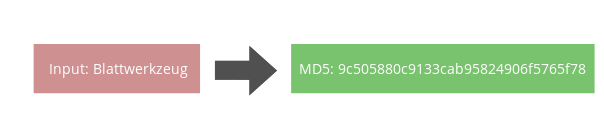
\includegraphics[scale=2]{hash.png}\par\bigskip
                        \todo[inline]{Allgemein: Kein Bild ohne Bildunterschrift (figure), auf jedes Bild muss aus dem Text verwiesen werden (ref)}

			Aus diesem Grund werden sogenannte Salts, zufällig generierte Zeichenketten, an das Passwort angehängt und darauf folgend die Hashfunktion angewandt.

			\begin{center}
				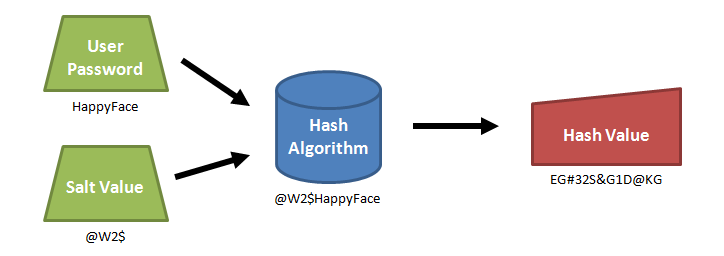
\includegraphics[scale=0.4]{salted_hash.png}
                        \end{center}
		\end{flushleft}

		\subsection{Sessions}
		\label{sec: sessions}

		\begin{flushleft}
			HTTP ein zustandsloses Protokoll, dass sich keine Informationen der jeweiligen Aufrufe zwischenspeichert. Dies ist unpraktisch, da so keine Informationen des Nutzers kurzzeitig gespeichert werden können\todo{Warum ist das ein Problem?}. \hlnote{Weshalb}{Am Satzanfang holprig} man auf die Session zurückgreifen kann. \par\bigskip


			Die Session ist eine serverseitige Daten \hlnote{speicher Möglichkeit}{Typo}. Dabei wird bei der Anfrage von einem Client an den Server ohne Session-ID eine Session und Session-ID erstellt. Diese Session-ID wird bei der Antwort des Servers mit an den Client ausgeliefert. Ab diesem Punkt wird bei jeder Anfrage vom Client an den Server die Session-ID mit gesendet. Dies kann über einen Cookie oder über die URI erfolgen. Aufgrund dessen kann der Server dem Client Daten aus der jeweiligen Session zur Verfügung stellen.

			\begin{center}
				will be replaced by useful graphic
				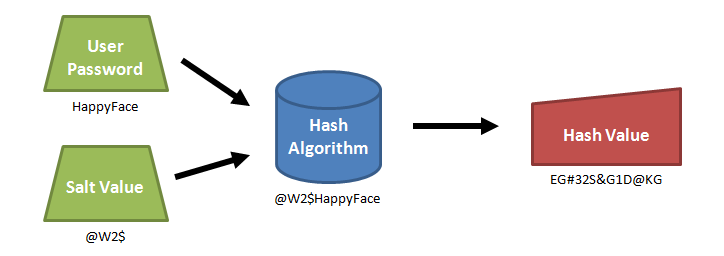
\includegraphics[scale=0.4]{salted_hash.png}
			\end{center}

		\end{flushleft}

		\subsection{JSON Web Token}
		\label{sec: jwt}
		\begin{flushleft}
			"JSON Web Token sind auf JSON basierende RFC 7519 genormte Access-Token." - Zitat Wikipedia, muss noch überarbeitet werden\par\bigskip

			 Diese Tokens werden zur eindeutigen Identifizierung von Nutzern verwendet und können die Session ersetzen. Dabei ist es bei einem JSON Web Token nicht von nöten die Daten auf dem Server zu speichern. Dies hat zur Folge, dass sich nicht um den Speicher \hlnote{gekümmert werden muss}{ugs}.\todo[inline]{Was sind Nachteile von JWT?} \par\bigskip

			Ein JSON Web Token besteht aus Header, Payload und Signatur. Dabei ist der Header und die Payload jeweils ein JSON Objekt.

			\subsubsection{Header}
			\label{sec: jwt_header}

			\begin{description}
				\leftskip=1em
				\item[typ] Der typ Claim beschreibt den Mediatypen des JWT, dieser wiederum teilt dem Client oder Server mit um welche Art von Medium an Daten es sich handelt\todo{Beispielwerte?}.
				\item[alg] Der alg Claim beschreibt die Verschlüsselungsmethode \todo{Beispielwerte?}
				\item[cty] Der cty Claim wird benötigt wenn der Payload des JSON Web Token ebenfalls ein JWT ist\todo{Wofür brauchst du das?}
			\end{description}

			IMAGE

			\subsubsection{Payload}
			\label{sec: jwt_payload}

			Die Payload beinhalteten Schlüssel-Wert Paare werden Claims genannt. Dabei handelt es sich um ein JSON Objekt, bei dem bestimmte Schlüssel des Objektes bereits reserviert sind. Diese nennen sich registrierte Claims. Außerdem gibt es öffentliche und private Claims. Hierbei wird zwischen öffentlichen und privaten differenziert.\par\bigskip


			\textbf{Beispiel registierter Claims}

			\begin{description}
				\leftskip=1em
				\item[iss]
				Der iss Claim steht für den Austeller des Tokens, beispielsweise eine Domain.
				\item[sub] Der sub Claim definiert für wen oder was diese Claims getätigt werden sollen.
				\item[aud] Der aud Claim wird genutzt um den Zugriff auf das Token auf eine bestimmte Domäne zu beschränken.
				\item[exp] Der exp Claim kennzeichnet den JWT mit einem Ablaufdatum.
				\item[nbf] Der nbf Claim bestimmt ab welchem Datum der JWT gültig ist.
				\item[iat] Der iat Claim sagt aus wann dieser Claim erstellt wurde.
                        \end{description}

                        \todo[inline]{Mehr konkrete Beispiele, weniger Breite}

			\textbf{Beispiel öffentlicher Claims}

			IMAGE\par\bigskip


			\textbf{Beispiel privater Claims}

			IMAGE\par\bigskip


			\subsubsection{Signatur}
			\label{sec: jwt_signature}

			Um die Signatur zu erhalten muss die Payload und der Header Base64 kodiert werden. Außerdem müssen diese beiden kodierten Zeichenfolgen mit einem Punkt als Trennzeichen verknüpft werden. Darauf folgend wird eine Hashfunktion auf das jeweilige Ergebnis mit zusätzlich sicherer Zeichenfolge als Parameter angewandt. An dieser Stelle kann festgestellt werden ob der JWT verändert wurde. \todo[inline]{stimmt, aber wie?}\par\bigskip


			\subsubsection{Zusammengesetzes Token}
			\label{sec: jwt_result}
			Schlussendlich ergibt sich der JWT aus kodierten Header, kodierten Payload und der Signatur. Dabei steht der Header am Anfang. Darauf folgend mit einem Punkt getrennt die Payload und zum Schluss die Signatur, ebenfalls mit einem Punkt getrennt. \par\bigskip

			IMAGE


			\subsection{Ruby on Rails}
			\label{sec: rails}
			Ruby on Rails ein quelloffenes Webframework für die Programmiersprache Ruby. Das Webframework nutzt das MVC Muster und stellt bereits ein sehr umfangreiches CLI zur Verfügung. \hlnote{Mittels des generate Werkzeugs kann beispielsweise Model, View und Controller erstellt werden. Jeder dieser Komponenten wird automatisch in die erstellte Rails Anwendung eingebunden.}{Wo brauchst du das?} Außerdem stellt Rails eine umfangreiche Test-Architektur und einen Service zum versenden von Mails. Dabei kann der Inhalt der E-Mail im Textformat oder als HTML versendet werden.\todo{Zu kurz: Datenbank-Anbindung}

                        \todo[inline]{Nochmal in den eigenen Quelltext schauen: Welche Aspekte sind wirklich relevant?}

			\subsubsection{Controller\todo{Davor: Routen}}
			\label{sec: rails_controller}
			Der Controller dient hierbei zur Kapselung von bestimmten Prozessen. Jede Route verweist in irgendeiner Weise auf eine Controller Funktion. In der der jeweiligen Controller Funktion wird dann meistens mit einem Model interagiert. Es wird beispielsweise eine Benutzerberechtigung abgefragt und individuell auf die Berechtigung reagiert. Um auf die jeweilige Berechtigung zu reagieren gibt es mehrere Möglichkeiten. Eine der Möglichkeiten wäre, direkt ein View Template auf dem Server zu rendern und an den Client auszuliefern. Eine andere Möglichkeit wäre ein JSON Objekt zurück zu geben und darauf mit dem Client zu agieren.

			\subsubsection{Model}
			\label{sec: rails_model}
			Das Model spielt während dieser Thesis \hlnote{eine große Rolle}{weasel}. Es stellt jeweils eine Datenbanktabelle dar. Die Attribute des Models sind jeweilige Spalten der Datenbanktabelle. Jedes Model kann zusätzliche Funktionen beinhalten, die direkt auf den jeweiligen Datenbankeintrag angewandt werden kann. Außerdem bietet Rails die Möglichkeit die Beziehungen zwischen Datenbanktabellen direkt in den Modellen festzulegen.

                        \todo[inline]{Validierung? Beziehungen?}

			\subsubsection{View}
			\label{sec: rails_view}
			Die View stellt in Rails die Möglichkeit HTML Template auf dem Server zu rendern. Dabei kann beim rendern das HTML Template dynamisch verändert werden. Da diese Komponente während dieser Thesis keine Rolle gespielt hat, wird diese nicht weiter erläutert.\par\bigskip

			\subsection{Zusammenfassung}
			\label{sec: rails_resuemee}
			Schlussendlich wird über die Route auf den jeweiligen Controller zugegriffen. Dieser fragt in den meisten Fällen nach einem bestimmten Eintrag eines Models. Darauf folgend wird mit dem Ergebnis der Anfrage interagiert. Es werden Veränderungen oder abfragen bestimmter Daten getätigt. Danach wird ein Ergebnis dem Client ausgeliefert.






			\begin{center}
				\includegraphics[scale=0.4]{rails.png}
			\end{center}

			\subsection{Angular}
			\label{sec: angular}
			Angular ist ein TypeScript basiertes Front-End Webframework, dass in vielen fällen für SPAs verwendet wird. Das Webframework bietet verschiedene Möglichkeiten dynamisch Daten und Elemente des DOMs zu manipulieren oder auszutauschen\todo{Wesentlicher Vorteil: Klare Entwurfsmuster}.\par\bigskip

			Hierbei bietet Angular die Möglichkeit HTML, CSS und TypeScript in Komponenten zu kapseln. Das bedeutet, dass jede Komponente unabhängig von einer anderen Komponente arbeiten kann.\par\bigskip

			Zur kommunikation mit einem Server und/oder zum Datenaustausch zwischen unterschiedlichen Komponenten wird \hlnote{meistens}{Weasel, wann nicht?} ein Service verwendet. Diese Services werden beim laden der Module instaziert und dem Konstruktor der Komponente als instanziertes Objekt übergeben.\par\bigskip

			Zusätzlich bietet Angular außerdem die Möglichkeit eigene Module zu erstellen in denen dann beispielsweise Services und Komponenten zusätzlich abgekapselt werden können. \hlnote{Einer der Vorteile}{Weasel} die Angular gegenüber anderen JavaScript Frameworks hat, sind die bereits von Angular \hlnote{mitgelieferten Module}{Welche?}.

			\begin{center}
				
\includegraphics[scale=0.1]{angular.png}
			\end{center}

			\subsection{oAuth2}
			\label{sec: oauth}
			oAuth2 ist ein offenes \hlnote{nach RFC genormtes}{Warum ist RFC wichtig?} Protokoll welches verwendet wird um eine Authentifizierung einer Anwendung mittels \hlnote{dritt Anbieter}{Typo} zu ermöglichen. Hierbei wird der Nutzer zuerst auf die jeweilige Seite des \hlnote{dritt Anbieter}{Typo} weitergeleitet. Dort muss der Nutzer sich authentifizieren und den Zugriff auf die Daten seines Kontos bestätigen. Nachdem der Zugriff auf die Daten bestätigt wurde, erhält die jeweilige Anwendung von dem dritt Anbieter einen Autorisierungs-Token. Dieser Autorisierungs-Token wird darauf folgend von der Anwendung genutzt um einen Zugriffs-Token von dem dritt Anbieter zu erhalten. Dieser ermöglicht schlussendlich den Zugriff auf die spezifischen Nutzerdaten des dritt Anbieters.\par\bigskip

			IMAGE\todo[inline]{Kommt hier ein Bild von den ``wollen sie diese Daten weitergeben'' Dialogen?}\par\bigskip

			In Blattwerkzeug wird genau dieser umfangreiche Vorgang von Omniauth übernommen. Aus diesem Grund wird oAuth2 in dieser Thesis nicht weiter erläutert.

			\subsection{Omniauth}
			\label{sec: omniauth}
			Omniauth ist eine quelloffene Library für Ruby on Rails und ermöglicht einem, eine Anmeldung mittels unterschiedlicher Anbieter. \hlnote{Hierbei}{Wobei?} werden bereits viele Funktionen von Omniauth selber übernommen. Sobald der Nutzer sich bei dem jeweiligen Anbieter angemeldet hat, wird die Antwort des jeweiligen Anbieters automatisch über die von Omniauth festgelegte Route verarbeitet. Jedoch muss vorher das spezifische Gem des Anbieters für Omniauth installiert werden.\par\bigskip

			Omniauth selber verfügt nur über die Developer Strategie, diese ermöglicht eine Anmeldung ohne spezifische Überprüfung der angegebenen Daten. Das hat zur Folge, dass diese Art von Anmeldung auf keinen Fall im Produktiv System vorhanden sein darf. Die Developer Strategie erzeugt automatisch ein \hlnote{Formular zur Anmeldung eines Nutzers}{Das Formular als solches ist nicht relevant}.

			\begin{center}
				\includegraphics[scale=0.5]{developer_strategy.png}
			\end{center}

			Die Möglichkeit dieses Formular zu deaktivieren und sich ausschließlich über ein API mit der Developer Strategie anzumelden ist nicht gegeben\todo{$\rightarrow$Implementierung}.\par\bigskip


			\subsubsection{Omniauth Identity\todo{$\rightarrow$Implementierung}}
			\label{sec: omniauth_identity}
			Omniauth Identity ist eine Library zur Erweiterung von Omniauth. Mit Omniauth Identity ist intern ein Anbieter gegeben mit dem es möglich ist, sich zusätzlich mit einem Passwort zu registrieren und anzumelden. Eben so wie die Developer Strategy, bietet auch diese Library die Möglichkeit ein vorgefertigtes Formular für Anmeldung und Registrierung zu erstellen. Jedoch ist es bei dieser Library optional und eine auschließliche Kommunikation über ein API ist möglich.\par\bigskip



		\end{flushleft}




\end{document}
%%% Local Variables:
%%% mode: latex
%%% TeX-engine: xetex
%%% TeX-master: t
%%% End:
